\documentclass[aspectratio=169,11pt]{beamer}
\def\courseweek{7}
% Shared style for the Introduction to Information Geometry lecture slides.
% Compile the lecture .tex files from this directory.
\providecommand{\courseweek}{1}
\usepackage[T1]{fontenc}
\usepackage[utf8]{inputenc}
\usepackage[sc]{mathpazo}
\renewcommand{\sfdefault}{lmss}
\renewcommand{\ttdefault}{lmtt}
\usepackage{amsmath,amssymb,mathtools}
\usepackage{tikz}
\usetikzlibrary{arrows.meta,calc,positioning}
\usepackage{pgfplots}
\pgfplotsset{compat=1.18}
\usepackage{booktabs}

\definecolor{courseink}{HTML}{173749}
\definecolor{coursemuted}{HTML}{526674}
\definecolor{courseteal}{HTML}{0E7287}
\definecolor{coursecopper}{HTML}{B66B43}
\definecolor{courseline}{HTML}{D4E0E3}
\definecolor{coursepale}{HTML}{EFF5F5}

\setbeamercolor{normal text}{fg=courseink,bg=white}
\setbeamercolor{structure}{fg=courseteal}
\setbeamercolor{frametitle}{fg=courseink,bg=white}
\setbeamercolor{title}{fg=courseink}
\setbeamercolor{subtitle}{fg=coursemuted}
\setbeamercolor{block title}{fg=courseink,bg=white}
\setbeamercolor{block body}{fg=courseink,bg=white}
\setbeamercolor{alerted text}{fg=coursecopper}
\setbeamerfont{title}{family=\rmfamily,series=\bfseries,size=\fontsize{32}{37}}
\setbeamerfont{frametitle}{family=\rmfamily,series=\bfseries,size=\fontsize{26}{31}}
\setbeamerfont{normal text}{size=\fontsize{18}{22}}
\setbeamerfont{subtitle}{size=\fontsize{17}{21}}
\setbeamersize{text margin left=0.78cm,text margin right=0.78cm}
\setbeamertemplate{navigation symbols}{}
\setbeamertemplate{itemize items}[circle]
\setbeamertemplate{enumerate items}[default]
\setbeamertemplate{blocks}[default]
\setlength{\parskip}{0.22em}
\setbeamertemplate{footline}{%
  \leavevmode\hbox to \paperwidth{\hspace{.78cm}%
  {\color{coursemuted}\fontsize{8.5}{10}\selectfont Introduction to Information Geometry \hspace{.32cm} / \hspace{.32cm} Week \courseweek}%
  \hfill{\color{coursemuted}\fontsize{8.5}{10}\selectfont \insertframenumber\hspace{.17cm}/\hspace{.17cm}\inserttotalframenumber}\hspace{.78cm}}%
  \vskip.17cm
}
\setbeamertemplate{frametitle}{%
  \vspace{.13cm}
  \insertframetitle\par
  \vspace{.08cm}
}
\setbeamertemplate{title page}{%
  \vspace*{1.00cm}
  {\color{courseteal}\fontsize{10}{13}\selectfont\bfseries
  INTRODUCTION TO INFORMATION GEOMETRY\par}
  \vspace{.40cm}
  {\usebeamerfont{title}\usebeamercolor[fg]{title}\inserttitle\par}
  \vspace{.22cm}
  {\usebeamerfont{subtitle}\usebeamercolor[fg]{subtitle}\insertsubtitle\par}
  \vfill
  {\color{coursemuted}\fontsize{13}{16}\selectfont Christopher Lee\par}
  \vspace{.34cm}
}

\pgfplotsset{
  courseplot/.style={
    width=11.05cm,
    height=5.15cm,
    axis line style={coursemuted!75},
    tick style={coursemuted!65},
    ticklabel style={font=\scriptsize,color=coursemuted},
    label style={font=\normalsize,color=courseink},
    grid=major,
    major grid style={courseline!70,line width=.4pt},
    line width=1.45pt,
    legend style={font=\small,draw=none,fill=none,at={(.98,.03)},anchor=south east},
    clip=true
  }
}

\newcommand{\highlightmath}[1]{{\color{courseteal}#1}}
\newcommand{\thinrule}{\par\vspace{.25cm}{\color{courseline}\rule{\linewidth}{.8pt}}\par}

% A one-dimensional state space.  x=0 and x=1 are placed at 0 and 9 units.
\newcommand{\stateinterval}[1]{%
 \begin{tikzpicture}[x=1cm,y=1cm]
   \draw[courseink,line width=1.25pt] (0,0)--(9,0);
   \foreach \pos/\lab in {0/0,9/1} {
     \fill[courseink] (\pos,0) circle(2.7pt);
     \node[below=9pt,text=coursemuted] at (\pos,0) {\(\lab\)};
   }
   #1
 \end{tikzpicture}%
}

% Paired pages are separate frames in the PDF, with matching titles.
% Supply the whole frame body for each version; the instructor may edit them
% independently without changing overlay logic.
\newcommand{\coursepair}[3]{%
  \begin{frame}{#1}#2\end{frame}%
  \begin{frame}{#1}#3\end{frame}%
}

% Equilateral representation of the categorical simplex, in barycentric
% coordinates with vertices A=(0,0), B=(1,0), C=(1/2,sqrt(3)/2).
\newcommand{\coursesimplex}[1]{%
 \begin{tikzpicture}[scale=4.9]
  \fill[coursepale] (0,0)--(1,0)--(.5,.8660254)--cycle;
  \draw[courseink,line width=.65pt] (0,0)--(1,0)--(.5,.8660254)--cycle;
  \node[below left,font=\small] at (0,0) {A};
  \node[below right,font=\small] at (1,0) {B};
  \node[above,font=\small] at (.5,.8660254) {C};
  #1
 \end{tikzpicture}%
}

\title{Fisher Information and Scores}
\subtitle{Week 7 \(\cdot\) Lecture 1}
\date{}
\begin{document}
\begin{frame}[plain]\titlepage\end{frame}

\begin{frame}{A metric from the KL expansion}
For positive \(P=(p_i)\) and a small tangent displacement \(u\),
\[
D(P\|P+u)=\frac12\sum_i\frac{u_i^2}{p_i}+O(\|u\|^3).
\]
\vspace{.49cm}
The resulting Fisher inner product is
\[
\highlightmath{g_P(u,v)=\sum_i\frac{u_iv_i}{p_i}},
\qquad\sum_i u_i=\sum_i v_i=0.
\]
\end{frame}

\begin{frame}{Length depends on the base distribution}
For the Bernoulli family, a probability displacement \(dp\)
has squared length
\[
\highlightmath{ds^2=\frac{dp^2}{p(1-p)}}.
\]
\vspace{.47cm}
The same change in \(p\) carries more Fisher length near a boundary
than near \(p=\frac12\).
\end{frame}

\begin{frame}{The Bernoulli metric coefficient}
\vspace{-.23cm}
\begin{center}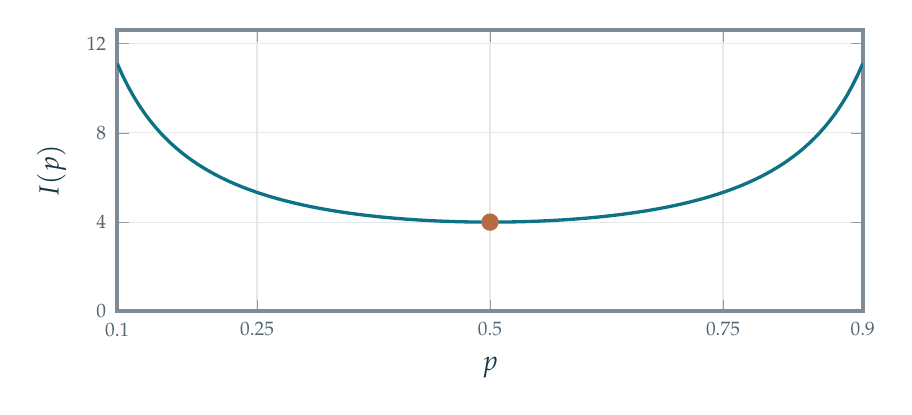
\begin{tikzpicture}
\begin{axis}[courseplot,xmin=.1,xmax=.9,ymin=0,ymax=12.6,
 xlabel={$p$},ylabel={$I(p)$},xtick={.1,.25,.5,.75,.9},
 ytick={0,4,8,12}]
\addplot[courseteal,very thick,domain=.1:.9,samples=140]{1/(x*(1-x))};
\addplot[only marks,coursecopper,mark=*,mark size=2.4pt]coordinates{(.5,4)};
\end{axis}\end{tikzpicture}\end{center}
\vspace{-.12cm}
Here \(I(p)=1/[p(1-p)]\); it is smallest at \(p=1/2\).
\end{frame}

\coursepair{A Fisher norm on the triangle}{
At \(P=(\frac12,\frac14,\frac14)\), consider
\(v=(0,.1,-.1)\).
\vspace{.4cm}
Find the squared Fisher norm
\[
g_P(v,v)=\sum_i\frac{v_i^2}{p_i}=\;?.
\]
}{
At \(P=(\frac12,\frac14,\frac14)\), consider
\(v=(0,.1,-.1)\).
\vspace{.4cm}
The squared norm is
\[
\highlightmath{g_P(v,v)=\frac{.01}{.25}+\frac{.01}{.25}=.08}.
\]
}

\begin{frame}{Scores describe parameter sensitivity}
Let \(P_\theta=(p_i(\theta))\) be a statistical family.
For observed outcome \(i\), the score is
\[
\highlightmath{S_\theta(i)=\frac{\partial}{\partial\theta}\ln p_i(\theta)}.
\]
\vspace{.44cm}
Its mean is zero:
\[
E_\theta[S_\theta]=\sum_i p_i\frac{p_i'}{p_i}=0.
\]
\end{frame}

\begin{frame}{Fisher information is score variance}
For a one-parameter family,
\[
\highlightmath{I(\theta)=E_\theta[S_\theta^2]
=\sum_i\frac{(p_i'(\theta))^2}{p_i(\theta)}}.
\]
\vspace{.46cm}
This is precisely the squared Fisher speed of the parameter curve.
\vspace{.4cm}
For several parameters, the expected score products form
the matrix \(G_{ab}=E[S_aS_b]\).
\end{frame}

\coursepair{Information in one Bernoulli observation}{
For outcomes \(0,1\), let \(P_p=(1-p,p)\).
\vspace{.35cm}
Find the two scores and then compute
\[
I(p)=E_p[S_p^2].
\]
\vspace{.35cm}
\[
S_p(1)=\;?,\quad S_p(0)=\;?,\quad I(p)=\;?.
\]
}{
For outcomes \(0,1\), let \(P_p=(1-p,p)\).
\vspace{.35cm}
The scores are \(\frac1p\) for outcome 1 and
\(-\frac1{1-p}\) for outcome 0.
\vspace{.35cm}
\[
\highlightmath{I(p)=p\left(\frac1p\right)^2
+(1-p)\left(\frac1{1-p}\right)^2=\frac1{p(1-p)}}.
\]
}

\begin{frame}{Information under a coordinate change}
Suppose \(\theta=\theta(\eta)\). The score obeys the chain rule.
\vspace{.46cm}
For a one-dimensional family,
\[
\highlightmath{I_\eta=I_\theta\left(\frac{d\theta}{d\eta}\right)^2}.
\]
\vspace{.45cm}
In several dimensions, with Jacobian \(J\),
\[
\highlightmath{G_\eta=J^T G_\theta J}.
\]
\end{frame}

\coursepair{Information in log-odds coordinates}{
Let \(L=\ln[p/(1-p)]\).
\vspace{.36cm}
Using \(dp/dL=p(1-p)\) and \(I_p=1/[p(1-p)]\),
find \(I_L\).
\vspace{.4cm}
\[
I_L=\;?.
\]
}{
Let \(L=\ln[p/(1-p)]\).
\vspace{.36cm}
The transformation law gives
\[
I_L=\frac1{p(1-p)}[p(1-p)]^2
=\highlightmath{p(1-p)}.
\]
\vspace{.4cm}
The metric coefficient changes with the coordinate.
}

\begin{frame}{Information accumulates in a sample}
For \(N\) independent observations, log likelihoods add.
Their score contributions have mean zero, so cross terms vanish:
\vspace{.48cm}
\[
\highlightmath{I_N(\theta)=N I(\theta)}.
\]
\vspace{.5cm}
The associated local statistical lengths scale by \(\sqrt N\).
\end{frame}

\begin{frame}{Cram\'{e}r--Rao and statistical precision}
Under the usual unbiasedness and differentiability hypotheses,
an estimator \(T\) of \(\theta\) satisfies
\[
\highlightmath{\operatorname{Var}_\theta(T)\geq\frac1{NI(\theta)}}.
\]
\vspace{.50cm}
For Bernoulli sampling, the empirical proportion has variance
\(p(1-p)/N\) and attains this bound.
\end{frame}

\coursepair{A lower bound for an estimator}{
Take \(N=100\) independent Bernoulli observations at \(p=0.2\).
\vspace{.4cm}
Compute \(I(p)\) and the Cram\'{e}r--Rao lower bound on variance:
\[
I(p)=\;?,\qquad\operatorname{Var}(T)\geq\;?.
\]
}{
Take \(N=100\) independent Bernoulli observations at \(p=0.2\).
\vspace{.4cm}
\[
\highlightmath{I(p)=\frac1{.2(.8)}=6.25}.
\]
\vspace{.28cm}
\[
\highlightmath{\operatorname{Var}(T)\geq\frac1{625}=.0016}.
\]
}

\begin{frame}{The same object in three languages}
\begin{itemize}\setlength{\itemsep}{.57cm}
\item The Hessian of local KL divergence defines a quadratic form.
\item Tangent vectors have lengths measured by that form.
\item A statistical score has expected square equal to the same length.
\end{itemize}
\end{frame}
\end{document}
